
%%--------------------------------------------------
%% CPO: Multiple Choice Questions
%%--------------------------------------------------


%% Chapter 20: Waves
%%--------------------------------------------------


%% Learning Objectives
%%--------------------------------------------------

%% Describe transverse and longitudinal waves. 
%% Learn the properties of waves. 
%% Calculate the speed of a wave. 
%% Identify the fundamental and harmonics of a standing wave. 
%% Learn how waves propagate.
%% Describe the four wave interactions. 
%% Describe the superposition principle and constructive and destructive interference. 
%% Review natural frequency and resonance. 
%% Explain the relationship between energy and its properties.


%% CPO Multiple Choice Questions
%%--------------------------------------------------
\element{cpo-mc}{
\begin{question}{cpo-ch20-q01}
    The term \emph{antinode} is another name for the:
    \begin{choices}
        \wrongchoice{fundamental frequency of an object.}
        \wrongchoice{harmonics of a vibrating string.}
        \wrongchoice{depression on a standing wave.}
      \correctchoice{``bump'' on a standing wave.}
    \end{choices}
\end{question}
}

\element{cpo-mc}{
\begin{question}{cpo-ch20-q02}
    Multiples of the fundamental frequency of a vibrating string are called:
    \begin{multicols}{2}
    \begin{choices}
      \correctchoice{harmonics}
        \wrongchoice{amplitudes}
        \wrongchoice{interferences}
        \wrongchoice{nodes}
    \end{choices}
    \end{multicols}
\end{question}
}

\element{cpo-mc}{
\begin{question}{cpo-ch20-q03}
    Which of the following is \emph{not} a property of waves?
    \begin{multicols}{2}
    \begin{choices}
        \wrongchoice{Frequency}
        \wrongchoice{Amplitude}
        \wrongchoice{Speed}
      \correctchoice{Weight}
    \end{choices}
    \end{multicols}
\end{question}
}

\element{cpo-mc}{
\begin{question}{cpo-ch20-q04}
    Under ordinary circumstances,
        a \rule[-0.1pt]{4em}{0.1pt} wave is the slowest wave.
    \begin{multicols}{2}
    \begin{choices}
        \wrongchoice{light}
        \wrongchoice{radio}
        \wrongchoice{sound}
      \correctchoice{water}
    \end{choices}
    \end{multicols}
\end{question}
}

\element{cpo-mc}{
\begin{question}{cpo-ch20-q05}
    The product of the frequency and the length of a wave yields its:
    \begin{multicols}{2}
    \begin{choices}
        \wrongchoice{period.}
        \wrongchoice{amplitude.}
        \wrongchoice{cycle.}
      \correctchoice{speed.}
    \end{choices}
    \end{multicols}
\end{question}
}

\element{cpo-mc}{
\begin{question}{cpo-ch20-q06}
    A sound wave, generated at a frequency of \SI{440}{\hertz} has a wavelength of \SI{2.3}{\meter} as it travels through a solid material.
    The approximate speed of the wave is:
    \begin{multicols}{2}
    \begin{choices}
        \wrongchoice{\SI{140}{\meter\per\second}}
        \wrongchoice{\SI{190}{\meter\per\second}}
        \wrongchoice{\SI{760}{\meter\per\second}}
      \correctchoice{\SI{1 000}{\meter\per\second}}
    \end{choices}
    \end{multicols}
\end{question}
}

\element{cpo-mc}{
\begin{question}{cpo-ch20-q07}
    Vibrating strings and similar systems have resonance patterns that occur at:
    \begin{choices}
        \wrongchoice{frequency intervals of \SI{12}{\hertz}.}
        \wrongchoice{amplitude intervals of \SI{1}{\meter}.}
      \correctchoice{multiples of the fundamental frequency.}
        \wrongchoice{frequency intervals equal to wave speed times wavelength.}
    \end{choices}
\end{question}
}

\newcommand{\myChapterTwentyWave}{
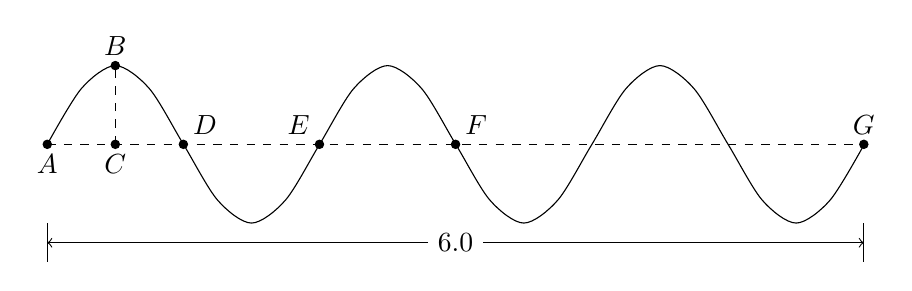
\begin{tikzpicture}[x=0.0454\textwidth]
    %% Graph
    \draw[domain=0:6*pi,smooth] plot (\x, {sin(\x r)});
    \draw[dashed] (0,0) to (18.84,0);
    %% Labels
    \node[anchor=north]     at (0,0)    {$A$};
    \node[anchor=south]     (B) at (1.57,1) {$B$};
    \node[anchor=north]     (C) at (1.57,0) {$C$};
        \draw[dashed]   (C) to (B);
    \node[anchor=south west]at (3.14,0) {$D$};
    \node[anchor=south east]at (6.28,0) {$E$};
    \node[anchor=south west]at (9.42,0) {$F$};
    \node[anchor=south]     at (18.84,0){$G$};
    %% Points
    \draw[fill] (0,0)   circle [radius=1.5pt];
    \draw[fill] (1.57,1) circle [radius=1.5pt];
    \draw[fill] (1.57,0) circle [radius=1.5pt];
    \draw[fill] (3.14,0) circle [radius=1.5pt];
    \draw[fill] (6.28,0) circle [radius=1.5pt];
    \draw[fill] (9.42,0) circle [radius=1.5pt];
    \draw[fill] (18.84,0) circle [radius=1.5pt];
    %% Length
    \node[anchor=center] (L)    at (9.42,-1.25) {\SI{6.0}{\meter}};
    \draw (0,-1.00) to (0,-1.50);
    \draw (18.84,-1.00) to (18.84,-1.50);
    \draw[->] (L) to (18.84,-1.25);
    \draw[->] (L) to  (0.00,-1.25);
\end{tikzpicture}
}

\element{cpo-mc}{
\begin{question}{cpo-ch20-q08}
    The diagram below represents a wave pattern in a certain medium.
    \begin{center}
        \myChapterTwentyWave
    \end{center}
    The wavelength in the diagram is represented by the distance from:
    \begin{multicols}{2}
    \begin{choices}
        \wrongchoice{$A$ to $D$.}
        \wrongchoice{$B$ to $C$.}
      \correctchoice{$D$ to $F$.}
        \wrongchoice{$F$ to $G$.}
    \end{choices}
    \end{multicols}
\end{question}
}

\element{cpo-mc}{
\begin{question}{cpo-ch20-q09}
    The diagram below represents a wave pattern in a certain medium.
    \begin{center}
        \myChapterTwentyWave
    \end{center}
    The distance from point $A$ to point $G$ is \SI{6.0}{\meter}.
    If the speed of the wave is \SI{330}{\meter\per\second},
        the frequency of this wave is:
    \begin{multicols}{2}
    \begin{choices}
        \wrongchoice{\SI{55}{\hertz}}
      \correctchoice{\SI{165}{\hertz}}
        \wrongchoice{\SI{660}{\hertz}}
        \wrongchoice{\SI{1 980}{\hertz}}
    \end{choices}
    \end{multicols}
\end{question}
}

\element{cpo-mc}{
\begin{question}{cpo-ch20-q10}
    A student does an experiment with a string vibrating at \SI{20}{\hertz} and observes the resonance pattern shown in the diagram:
    \begin{center}
    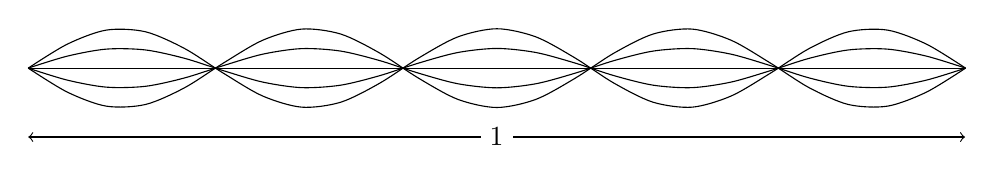
\begin{tikzpicture}[x=0.0625\columnwidth,yscale=0.5]
        \draw[domain=0:5*pi,smooth,thin] plot (\x, {0.50*sin(\x r)});
        \draw[domain=0:5*pi,smooth,thin] plot (\x, {-0.5*sin(\x r)});
        \draw[domain=0:5*pi,smooth,thin] plot (\x, {1.00*sin(\x r)});
        \draw[domain=0:5*pi,smooth,thin] plot (\x, {-1.0*sin(\x r)});
        \draw[thin] (0,0) -- (15.7,0);
        \draw[<->] (0,-1.75) -- (15.7,-1.75)
            node[pos=0.5,fill=white] {\SI{1}{\meter}};
    \end{tikzpicture}
    \end{center}
    The speed of the wave on the string is:
    \begin{multicols}{2}
    \begin{choices}
        \wrongchoice{\SI{4.0}{\meter\per\second}}
      \correctchoice{\SI{8.0}{\meter\per\second}}
        \wrongchoice{\SI{20}{\meter\per\second}}
        \wrongchoice{\SI{100}{\meter\per\second}}
    \end{choices}
    \end{multicols}
\end{question}
}

\element{cpo-mc}{
\begin{question}{cpo-ch20-q11}
    The wavelength of a certain frequency of light is \SI{5e-7}{\meter}.
    If the speed of light is \SI{300 000}{\kilo\meter\per\second},
        the frequency of the light is:
    \begin{multicols}{2}
    \begin{choices}
        \wrongchoice{\SI{1.67e-15}{\hertz}}
        \wrongchoice{\SI{1.67e-12}{\hertz}}
        \wrongchoice{\SI{6.00e11}{\hertz}}
      \correctchoice{\SI{6.00e14}{\hertz}}
    \end{choices}
    \end{multicols}
\end{question}
}

\element{cpo-mc}{
\begin{question}{cpo-ch20-q12}
    The bending of a wave front around a barrier is called:
    \begin{multicols}{2}
    \begin{choices}
        \wrongchoice{reflection}
      \correctchoice{refraction}
        \wrongchoice{diffraction}
        \wrongchoice{absorption}
    \end{choices}
    \end{multicols}
\end{question}
}

\element{cpo-mc}{
\begin{question}{cpo-ch20-q13}
    If your fingertip repeatedly touches the surface of water in a container at regular intervals,
        the action will produce:
    \begin{multicols}{2}
    \begin{choices}
        \wrongchoice{plane waves}
      \correctchoice{circular waves}
        \wrongchoice{crest only}
        \wrongchoice{troughs only}
    \end{choices}
    \end{multicols}
\end{question}
}

\element{cpo-mc}{
\begin{question}{cpo-ch20-q14}
    The diagram represents a wave interaction as wave fronts pass through a small opening.
    \begin{center}
    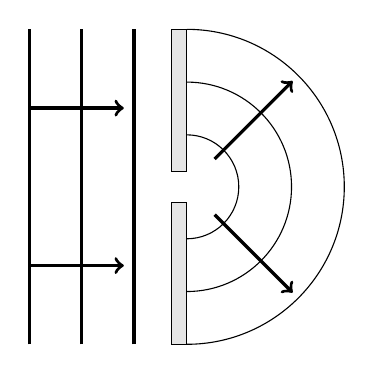
\begin{tikzpicture}
        %% Incoming
        \foreach \i in {0,0.66,1.33} {
            \draw[very thick] (\i,0) -- (\i,4);
        }
        \draw[very thick,->] (0,3) -- (1.2,3);
        \draw[very thick,->] (0,1) -- (1.2,1);
        %% Barrier
        \draw[fill=white!90!black] (1.8,0) rectangle (2,1.8);
        \draw[fill=white!90!black] (1.8,2.2) rectangle (2,4);
        %% Outgoing
        \foreach \i in {0.66,1.33,2.00} {
            \draw[] (2,2)++(90:\i) arc (90:-90:\i);
        }
        \draw[very thick,->] (2,2)++(-45:0.5) --++ (-45:1.4);
        \draw[very thick,->] (2,2)++(+45:0.5) --++ (+45:1.4);
    \end{tikzpicture}
    \end{center}
    This is an example of:
    \begin{multicols}{2}
    \begin{choices}
      \correctchoice{diffraction}
        \wrongchoice{refraction}
        \wrongchoice{reflection}
        \wrongchoice{absorption}
    \end{choices}
    \end{multicols}
\end{question}
}

\element{cpo-mc}{
\begin{question}{cpo-ch20-q15}
    As a wave front crosses a boundary between two different media,
        the wave front may change direction, an interaction known as:
    \begin{multicols}{2}
    \begin{choices}
        \wrongchoice{reflection}
      \correctchoice{refraction}
        \wrongchoice{diffraction}
        \wrongchoice{absorption}
    \end{choices}
    \end{multicols}
\end{question}
}

\element{cpo-mc}{
\begin{question}{cpo-ch20-q16}
    Theaters often use heavy curtains to reduce echoes during performances.
    The function of the curtains is to:
    \begin{multicols}{2}
    \begin{choices}
        \wrongchoice{refract sound}
        \wrongchoice{refract sound}
        \wrongchoice{diffract sound}
      \correctchoice{absorb sound}
    \end{choices}
    \end{multicols}
\end{question}
}

\element{cpo-mc}{
\begin{question}{cpo-ch20-q17}
    Diffraction causes waves to:
    \begin{choices}
        \wrongchoice{bounce off hard surfaces}
      \correctchoice{spread out through small openings}
        \wrongchoice{become smaller as they move}
        \wrongchoice{increase their frequency}
    \end{choices}
\end{question}
}

\element{cpo-mc}{
\begin{question}{cpo-ch20-q18}
    The process by which the amplitude of waves is reduced as a wave loses energy while moving through a substance is called:
    \begin{multicols}{2}
    \begin{choices}
        \wrongchoice{reflection}
        \wrongchoice{diffraction}
      \correctchoice{absorption}
        \wrongchoice{refraction}
    \end{choices}
    \end{multicols}
\end{question}
}

\element{cpo-mc}{
\begin{question}{cpo-ch20-q19}
    The direction a wave moves is:
    \begin{choices}
        \wrongchoice{parallel to the waves fronts}
      \correctchoice{perpendicular to the wave fronts}
        \wrongchoice{in the direction of increasing amplitude}
        \wrongchoice{in the direction of decreasing frequency}
    \end{choices}
\end{question}
}

\element{cpo-mc}{
\begin{question}{cpo-ch20-q20}
    You are still able to hear sounds coming from a room when the door is open only a tiny crack due to:
    \begin{multicols}{2}
    \begin{choices}
        \wrongchoice{reflection}
        \wrongchoice{refraction}
      \correctchoice{diffraction}
        \wrongchoice{absorption}
    \end{choices}
    \end{multicols}
\end{question}
}

\element{cpo-mc}{
\begin{question}{cpo-ch20-q21}
    Waves are affect by boundaries.
    When a wave front meets a certain boundary,
        all of the following may occur \emph{except} a change:
    \begin{choices}
        \wrongchoice{of direction}
        \wrongchoice{in the patter of the wave front}
      \correctchoice{of frequency}
        \wrongchoice{of amplitude}
    \end{choices}
\end{question}
}

\element{cpo-mc}{
\begin{questionmult}{ch20-Q22}
    Two large waves on the ocean come together on the ocean's surface to form a gigantic wave.
    The interaction responsible for this is called:
    \begin{choices}
        \wrongchoice{frequency amplification}
      \correctchoice{constructive interference}
        \wrongchoice{destructive interference}
        \wrongchoice{amplitude destruction}
    \end{choices}
\end{questionmult}
}

\element{cpo-mc}{
\begin{question}{cpo-ch20-q23}
    Devices like a guitar, a piano,
        and a microwave oven function using controlled:
    \begin{choices}
      \correctchoice{standing waves}
        \wrongchoice{destructive interference}
        \wrongchoice{frequency amplification}
        \wrongchoice{amplitude reduction}
    \end{choices}
\end{question}
}

\element{cpo-mc}{
\begin{question}{cpo-ch20-q24}
    Resonance in waves is created by:
    \begin{choices}
        \wrongchoice{longitudinal waves only.}
        \wrongchoice{constructive interference with a wave's own reflection.}
      \correctchoice{diffraction of a wave around an object.}
        \wrongchoice{absorption as a wave crosses a boundary.}
    \end{choices}
\end{question}
}

\element{cpo-mc}{
\begin{question}{cpo-ch20-q25}
    The natural frequency of a guitar string can be changed using any of the following means \emph{except}:
    \begin{choices}
        \wrongchoice{increasing the length of the string.}
      \correctchoice{plucking the string with greater force.}
        \wrongchoice{increasing the thickness of the string.}
        \wrongchoice{decreasing the length of the string.}
    \end{choices}
\end{question}
}

\element{cpo-mc}{
\begin{question}{cpo-ch20-q26}
    Which wave interaction could be demonstrated by a single wave pulse?
    \begin{choices}
        \wrongchoice{A standing wave}
      \correctchoice{Reflection}
        \wrongchoice{Constructive interference}
        \wrongchoice{The superposition principle}
    \end{choices}
\end{question}
}

\element{cpo-mc}{
\begin{question}{cpo-ch20-q27}
    Which pair of moving pulses on a rope will produce destructive interference?
    \begin{multicols}{2}
    \begin{choices}
        \AMCboxDimensions{down=-0.95cm}
        \correctchoice{
            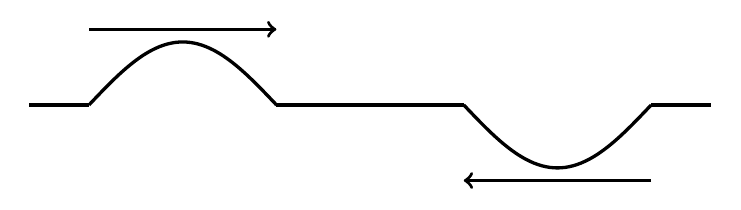
\begin{tikzpicture}[x=0.0625\columnwidth,yscale=0.8]
                \draw[draw=white] (-1.00,-1.2) rectangle (9.42,1.2);
                %% Wave Rope
                \draw[domain=0:pi,smooth,very thick] plot (\x, {sin(\x r)});
                \draw[domain=0:pi,smooth,very thick] plot (\x+6.28, {-1*sin(\x r)});
                %% Arrows
                \draw[very thick,->] (0,1.2) to (3.14,1.2);
                \draw[very thick,->] (9.42,-1.2) to (6.28,-1.2);
                %% Flat Rope
                \draw[very thick] (-1,0) to (0,0);
                \draw[very thick] (3.14,0) to (6.28,0);
                \draw[very thick] (9.42,0) to (10.42,0);
            \end{tikzpicture}
        }
        \wrongchoice{
            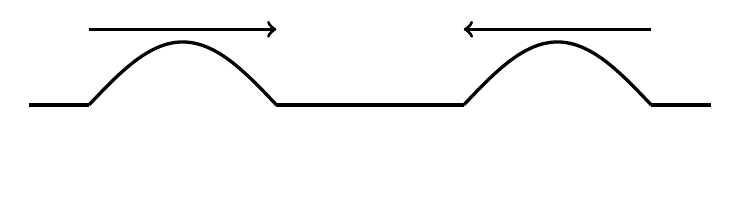
\begin{tikzpicture}[x=0.0625\columnwidth,yscale=0.8]
                \draw[draw=white] (-1.00,-1.2) rectangle (9.42,1.2);
                %% Wave Rope
                \draw[domain=0:pi,smooth,very thick] plot (\x, {sin(\x r)});
                \draw[domain=0:pi,smooth,very thick] plot (\x+6.28, {sin(\x r)});
                %% Arrows
                \draw[very thick,->] (0,1.2) to (3.14,1.2);
                \draw[very thick,->] (9.42,1.2) to (6.28,1.2);
                %% Flat Rope
                \draw[very thick] (-1,0) to (0,0);
                \draw[very thick] (3.14,0) to (6.28,0);
                \draw[very thick] (9.42,0) to (10.42,0);
            \end{tikzpicture}
        }
        \wrongchoice{
            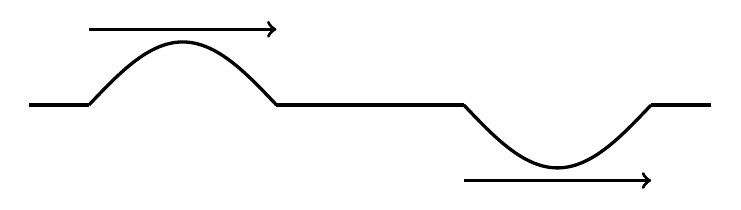
\begin{tikzpicture}[x=0.0625\columnwidth,yscale=0.8]
                \draw[draw=white] (-1.00,-1.2) rectangle (9.42,1.2);
                %% Wave Rope
                \draw[domain=0:pi,smooth,very thick] plot (\x, {sin(\x r)});
                \draw[domain=0:pi,smooth,very thick] plot (\x+6.28, {-1*sin(\x r)});
                %% Arrows
                \draw[very thick,->] (0,1.2) to (3.14,1.2);
                \draw[very thick,->] (6.28,-1.2) to (9.42,-1.2) ;
                %% Flat Rope
                \draw[very thick] (-1,0) to (0,0);
                \draw[very thick] (3.14,0) to (6.28,0);
                \draw[very thick] (9.42,0) to (10.42,0);
            \end{tikzpicture}
        }
        \wrongchoice{
            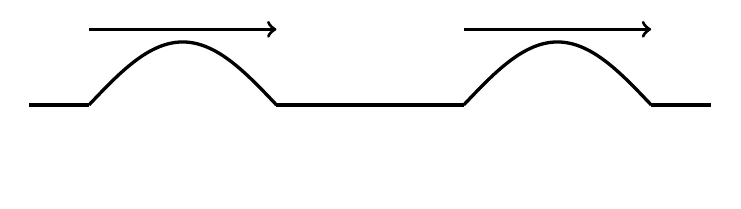
\begin{tikzpicture}[x=0.0625\columnwidth,yscale=0.8]
                \draw[draw=white] (-1.00,-1.2) rectangle (9.42,1.2);
                %% Wave Rope
                \draw[domain=0:pi,smooth,very thick] plot (\x, {sin(\x r)});
                \draw[domain=0:pi,smooth,very thick] plot (\x+6.28, {sin(\x r)});
                %% Arrows
                \draw[very thick,->] (0,1.2) to (3.14,1.2);
                \draw[very thick,->] (6.28,1.2) to (9.42,1.2) ;
                %% Flat Rope
                \draw[very thick] (-1,0) to (0,0);
                \draw[very thick] (3.14,0) to (6.28,0);
                \draw[very thick] (9.42,0) to (10.42,0);
            \end{tikzpicture}
        }
    \end{choices}
    \end{multicols}
\end{question}
}

\element{cpo-mc}{
\begin{question}{cpo-ch20-q28}
    Two pulses are traveling along a string toward each other as represented in the diagram below:
    \begin{center}
    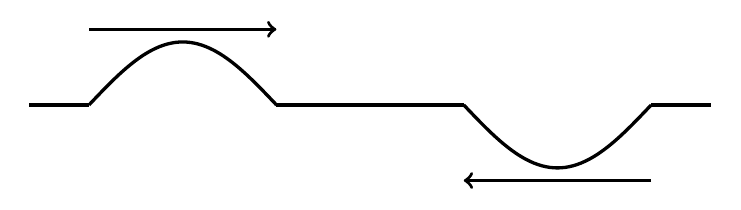
\begin{tikzpicture}[x=0.0625\textwidth,yscale=0.8]
        %% Wave Rope
        \draw[domain=0:pi,smooth,very thick] plot (\x, {sin(\x r)});
        \draw[domain=0:pi,smooth,very thick] plot (\x+6.28, {-1*sin(\x r)});
        %% Arrows
        \draw[very thick,->] (0,1.2) to (3.14,1.2);
        \draw[very thick,->] (9.42,-1.2) to (6.28,-1.2);
        %% Flat Rope
        \draw[very thick] (-1,0) to (0,0);
        \draw[very thick] (3.14,0) to (6.28,0);
        \draw[very thick] (9.42,0) to (10.42,0);
    \end{tikzpicture}
    \end{center}
    Which phenomenon will occur as the pulses meet?
    \begin{multicols}{2}
    \begin{choices}
      \correctchoice{Interference}
        \wrongchoice{Diffraction}
        \wrongchoice{Reflection}
        \wrongchoice{Refraction}
    \end{choices}
    \end{multicols}
\end{question}
}

\element{cpo-mc}{
\begin{question}{cpo-ch20-q29}
    Maximum destructive interference between two waves will occur when the waves are out of phase by:
    \begin{multicols}{4}
    \begin{choices}
      \correctchoice{\ang{45}}
        \wrongchoice{\ang{90}}
        \wrongchoice{\ang{180}}
        \wrongchoice{\ang{360}}
    \end{choices}
    \end{multicols}
\end{question}
}

\element{cpo-mc}{
\begin{question}{cpo-ch20-q30}
    Which pair of waves produces a resultant wave with the largest amplitude?
    \begin{multicols}{2}
    \begin{choices}
        \AMCboxDimensions{down=-0.5cm}
        \wrongchoice{
            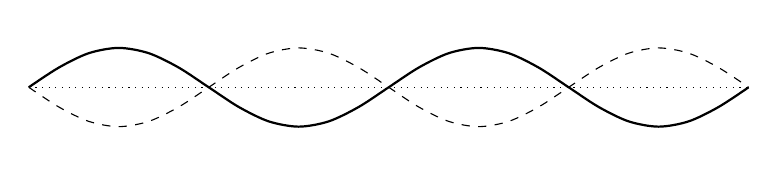
\begin{tikzpicture}[x=0.06\columnwidth,yscale=0.5]
                \draw[draw=white] (0,-1.5) to (12.56,1.5);
                %% Graph
                \draw[domain=0:4*pi,smooth,thick] plot (\x, {sin(\x r)});
                \draw[domain=0:4*pi,smooth,dashed] plot (\x, {-1*sin(\x r)});
                \draw[dotted] (0,0) to (12.56,0);
            \end{tikzpicture}
        }
        \correctchoice{
            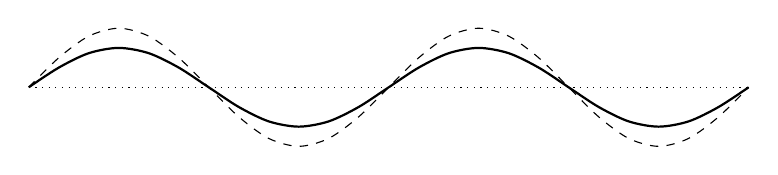
\begin{tikzpicture}[x=0.06\columnwidth,yscale=0.5]
                \draw[draw=white] (0,-1.5) to (12.56,1.5);
                %% Graph
                \draw[domain=0:4*pi,smooth,thick] plot (\x, {sin(\x r)});
                \draw[domain=0:4*pi,smooth,dashed] plot (\x, {1.5*sin(\x r)});
                \draw[dotted] (0,0) to (12.56,0);
            \end{tikzpicture}
        }
        \wrongchoice{
            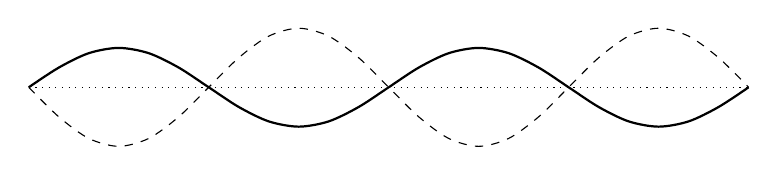
\begin{tikzpicture}[x=0.06\columnwidth,yscale=0.5]
                \draw[draw=white] (0,-1.5) to (12.56,1.5);
                %% Graph
                \draw[domain=0:4*pi,smooth,thick] plot (\x, {sin(\x r)});
                \draw[domain=0:4*pi,smooth,dashed] plot (\x, {-1.5*sin(\x r)});
                \draw[dotted] (0,0) to (12.56,0);
            \end{tikzpicture}
        }
        \wrongchoice{
            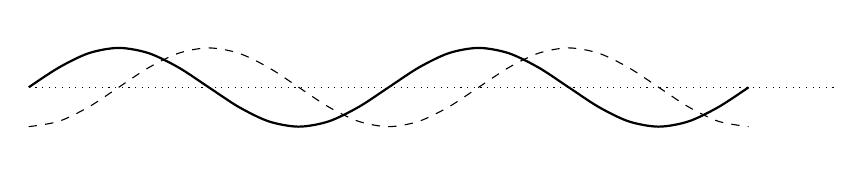
\begin{tikzpicture}[x=0.06\columnwidth,yscale=0.5]
                \draw[draw=white] (0,-1.5) to (12.56,1.5);
                %% Graph
                \draw[domain=0:4*pi,smooth,thick] plot (\x, {sin(\x r)});
                \draw[domain=-0.5*pi:3.5*pi,smooth,dashed] plot (\x+1.57, {sin(\x r)});
                \draw[dotted] (0,0) to (14.13,0);
            \end{tikzpicture}
        }
    \end{choices}
    \end{multicols}
\end{question}
}

\element{cpo-mc}{
\begin{question}{cpo-ch20-q31}
    Maximum constructive interference between two waves of the same frequency could occur when their phase difference is:
    \begin{multicols}{4}
    \begin{choices}
        \wrongchoice{$\dfrac{3\lambda}{2}$}
        \wrongchoice{$\dfrac{\lambda}{2}$}
        \wrongchoice{$\dfrac{\lambda}{4}$}
      \correctchoice{$\lambda$}
    \end{choices}
    \end{multicols}
\end{question}
}

\element{cpo-mc}{
\begin{question}{cpo-ch20-q32}
    For a standing wave to form in a medium, two waves must:
    \begin{choices}
        \wrongchoice{travel in the same direction.}
        \wrongchoice{have difference wavelengths.}
      \correctchoice{have the same frequency.}
        \wrongchoice{have difference amplitudes.}
    \end{choices}
\end{question}
}

\endinput


